\documentclass[a4paper,11pt,uplatex]{jsarticle}


% 数式
\usepackage{amsmath,amsfonts}
\usepackage{bm}
\usepackage{physics}
% 画像
\usepackage[dvipdfmx]{graphicx}
\usepackage[dvipdfmx,colorlinks=true,linkcolor=blue]{hyperref}
\usepackage{pxjahyper}

\begin{document}


\section{Principle}
\subsection{アンジュレータ放射光}
アンジュレータの原理を以下に示す。アンジュレータによって発生した周期的磁場中を電子ビームが通過すると、電子が蛇行("undulate")する。
磁場による加速度運動に伴いシンクロトロン放射光が発生する。
磁場周期と電子ビームエネルギーに依存して、発生する放射光は特定の波長に強いピークを持つ。
この特性はアンジュレータのK値と呼ばれる以下の特徴量によって表現できる。
$\text{K} \simeq 1$の時をアンジュレータと呼び準単色光が得られるが、$\text{K} \gg 1$の時には広い波長にわたって等間隔にピークを持つような放射光が発生し、このような挿入光源をウィグラーと呼ぶ。
アンジュレータ放射光の時間構造は以下に示すようなパルス型であることが知られている。
\subsection{アンジュレータ放射光 - タンデムアンジュレータ}
アンジュレータを電子ビームに沿って2つ連結した構成は放射光科学において広く使われている。
これらのアンジュレータ間にシケイン電磁石を配置することで遅延を調整することが可能になる。
\subsection{干渉の原理}
タンデム型アンジュレータから放射される放射光はダブルパルス型の波形となる。
回折格子のそれぞれの格子から散乱された光は格子間隔に比例して遅延された光の干渉となる。
そのためダブルパルスの二つのパルスは格子に寄る遅延を受けて干渉できることになる。
\subsection{電子ビームエネルギーと干渉光周期の関係式}
ダブルパルスの間隔は以下のような近似で理解することができる。
上流のアンジュレータで発生する放射光は電子ビームよりも早く、電子が下流側のアンジュレータに到達した時にはアンジュレータ間の距離に比例した時間差が生じる。
\begin{eqnarray}
  \Delta = \frac{1}{2\gamma^2}d \label{path shift}
\end{eqnarray}
この時間差は放射光の2つのパルスの位相差となる。
\begin{eqnarray}
  \Phi = \frac{2\pi\Delta}{\lambda_L}
\end{eqnarray}
位相差に対応して干渉光は強めあい、干渉光強度は
\begin{eqnarray}
  |\tilde{E} \left( 1+ e^{i\Phi}\right)|^2 
&= |\tilde{E}|^2 \left( 1 + \cos(\Phi) \right)\\
&= |\tilde{E}|^2 \left( 1 + \cos(\frac{2\pi}{2\gamma^2\lambda_L}d) \right) 
  \label{oscillation}
\end{eqnarray}
これより、dを変化させると干渉光の位相差が変化し強度が周期的に変動することがわかる。
式(\ref{oscillation})から、アンジュレータ間距離を$2\gamma^2\lambda_L$だけ動かした時に1周する。
この周期を$\lambda_{osc}$とおけば$\gamma$および電子ビームエネルギーが
\begin{eqnarray}
  \gamma = \sqrt{\frac{\lambda_{\text{osc}}}{2\lambda_L}}\\
  \text{E}_\text{beam} =m_e c^2  \sqrt{\frac{\lambda_{\text{osc}}}{2\lambda_L}} 
\end{eqnarray}
すなわち、干渉光の波長$\lambda_L$と、アンジュレータ間距離を変動させた時の干渉光の変動の周期$\lambda_{\text{osc}}$
を精密に測定することで電子ビームエネルギーが精密に測定できる。
\subsection{補正 - 放射角度と干渉光周期の関係式}
式(\ref*{path shift})は放射光角度が電子ビームの光路差である。
電子ビームの軸と放射光の放射角(近似的に放射光の観測角)を$\theta$とおくと、
アンジュレータ間の距離$d$と$\theta$で光路差が$d(1-\cos{\theta})$と表される。
これと電子ビームの遅延による光路差の両方を考慮した光路差は、
\begin{eqnarray}
  \Delta &= d\frac{1}{2\gamma^2} + d(1 - \cos{\theta}) \\
          &= d(\frac{1}{2\gamma^2} + \frac{\theta^2}{2})\\
\end{eqnarray}
と表せる。したがって放射光の観測角($\simeq$ 放射角)の補正を入れることで干渉光の周期は
\begin{eqnarray}
  \lambda_{\text{osc}} = \frac{\lambda_L}{\frac{1}{2\gamma^2} + \frac{\theta^2}{2}}
\end{eqnarray}
となる。ある観測角$\theta$では、













\clearpage

\begin{figure}[tb]
  \centering
  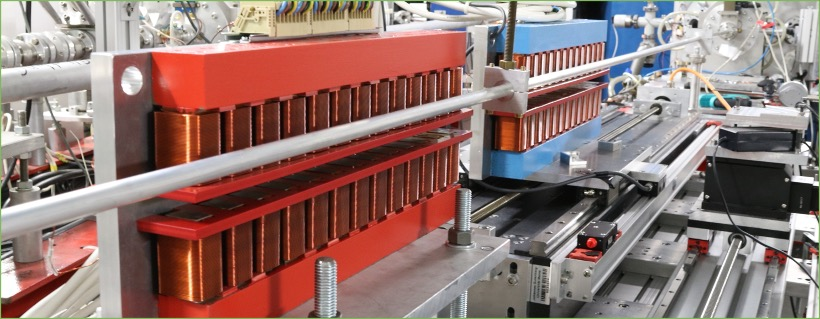
\includegraphics[width=0.8\linewidth]{image/1-1.jpg}\\
  \caption{サンプルの図}
  \label{sample_image}
\end{figure}

\begin{itemize}
  \item a
\end{itemize}
\begin{enumerate}
  \item b
\end{enumerate}

\begin{align}
\frac{1}{2} = \qty(\frac{1}{3}) + \qty{1}\Sigma
\end{align}
\end{document}
